% !TeX TS-program = pdflatex

\documentclass[a4paper,12pt]{book} % Layout dubbelzijdig
\usepackage{tikz} % Nodig voor voorkant
\usepackage[outer=3.0cm,top=3cm,inner=2.0cm,bottom=3cm,bindingoffset=0.5cm,marginparwidth=5mm,marginparsep=5mm]{geometry} % Instellen pagina-opmaak
\usepackage[T1]{fontenc}
\usepackage[sfdefault,lining]{FiraSans}
\usepackage{newtxsf}
\usepackage{kantlipsum} % Makkelijk proeftekst
\usepackage[dutch]{babel} % Nederlands als taal
\usepackage{parskip} % Niet inspringen en ruimte tussen alinea's
\usepackage[onehalfspacing]{setspace} % Regelafstand 1.5
\usepackage{booktabs} % mooi afgewerkte tabellen

%% Clear header and footer for blank pages, possibly print "This page ..."
%\newcommand{\thispageintentionallyleftblank}{Deze pagina is opzettelijk leeg gelaten}
\newcommand{\thispageintentionallyleftblank}{}
\makeatletter
\renewcommand*{\cleardoublepage}{\clearpage\if@twoside \ifodd\c@page\else
\hbox{}\vfill\begin{center}\thispageintentionallyleftblank\end{center}\vfill\vfill%
\thispagestyle{empty}%
\newpage%
\if@twocolumn\hbox{}\newpage\fi\fi\fi}
\makeatother

%% Create clickable (hyper)links
%% http://mirror.koddos.net/CTAN/macros/latex/contrib/hyperref/doc/manual.pdf
\usepackage{hyperref}
\hypersetup{
%    plainpages=false,
    breaklinks=true,
    colorlinks=true,
    linkcolor=black,
    linkcolor=black,
    citecolor=black,
    urlcolor=black,
    filecolor=black,
    pdfdisplaydoctitle=true,
    pdfstartview=FitH,
    pdfpagelayout=TwoPageRight,
}

% !!!apacite laden *na* hyerref!!!
\usepackage{apacite} % voor APA-style referenties
\bibliographystyle{apacite}

%% Change appearance of titles
%% http://archive.cs.uu.nl/mirror/CTAN/macros/latex/contrib/titlesec/titlesec.pdf
%\RequirePackage{titlesec}
%\RequirePackage{titletoc}
%\titleformat{\chapter}[hang]{\Huge\bfseries}{\thechapter.}{0.7em}{}
%\titleformat{\section}{\large\bfseries}{\thesection}{1em}{}
%\titleformat{\subsection}{\bfseries}{\thesubsection}{1em}{}
%\newlength{\aftersubtitle}
%\setlength{\aftersubtitle}{1.2\baselineskip}
%\newlength{\aftersubsection}
%\setlength{\aftersubsection}{\aftersubtitle}
%\addtolength{\aftersubsection}{-\baselineskip}
%\titlespacing*{\section}{0pt}{\baselineskip}{\aftersubsection}
%\titlespacing*{\subsection}{0pt}{.8\baselineskip}{\aftersubsection}
%\titlespacing*{\subsubsection}{0pt}{.6\baselineskip}{0pt}

%% Using fancy headers and footers
%% http://ftp.snt.utwente.nl/pub/software/tex/macros/latex/contrib/fancyhdr/fancyhdr.pdf
\usepackage{fancyhdr}
\pagestyle{fancy}
\addtolength{\headwidth}{\marginparsep}
\addtolength{\headwidth}{\marginparwidth}
\renewcommand{\chaptermark}[1]{\markboth{#1}{}}
\renewcommand{\sectionmark}[1]{\markright{\thesection\ #1}}
\fancyhf{}
\fancyhead[LE,RO]{\small\textbf{\thepage}}
\fancyhead[LO]{\small\textbf{\rightmark}}
\fancyhead[RE]{\small\textbf{\leftmark}}
\fancypagestyle{plain}{%
\fancyhead{} % get rid of headers
\renewcommand{\headrulewidth}{0pt} % and the line
}

%% Making captions nicer...
%% http://ftp.snt.utwente.nl/pub/software/tex/macros/latex/contrib/caption/caption-eng.pdf
%% http://mirror.koddos.net/CTAN/macros/latex/contrib/caption/subcaption.pdf
\RequirePackage[font=footnotesize,format=plain,labelfont=bf,textfont=sl]{caption}
\RequirePackage[labelformat=simple,font=footnotesize,format=plain,labelfont=bf,textfont=sl]{subcaption}
\captionsetup[figure]{justification=centering,singlelinecheck=off,belowskip=-1ex}
\captionsetup[table]{justification=centering,singlelinecheck=off,skip=1ex}
\captionsetup[subfigure]{justification=centering,singlelinecheck=off,skip=3pt}
\captionsetup[subtable]{justification=centering,singlelinecheck=off,skip=3pt}
%% Put parens around the subfig name (a) (b) etc.
\renewcommand\thesubfigure{(\alph{subfigure})}
\renewcommand\thesubtable{(\alph{subtable})}

\def\coverpagefontstudent{\fontsize{30}{40}\selectfont\normalfont}
\def\coverpagefontopleiding{\fontsize{20}{30}\selectfont\normalfont}
\def\coverpagefonttitle{\fontsize{40}{50}\selectfont\bfseries}
\def\coverpagefontisubtitle{\fontsize{25}{35}\selectfont\normalfont}
\def\coverpagefontthuas{\fontsize{40}{50}\scshape\selectfont}
\definecolor{thuasgreen}{RGB}{158,167,0}
\definecolor{thuasgrey}{RGB}{34,51,67}

\begin{document}
  %% The front page (or title page if you wish...)
  \thispagestyle{empty}
  \begin{tikzpicture}[remember picture,overlay]
      \node (image) [shape=rectangle,draw=none, minimum width=\paperwidth, minimum height=\paperheight] at (current page.center) {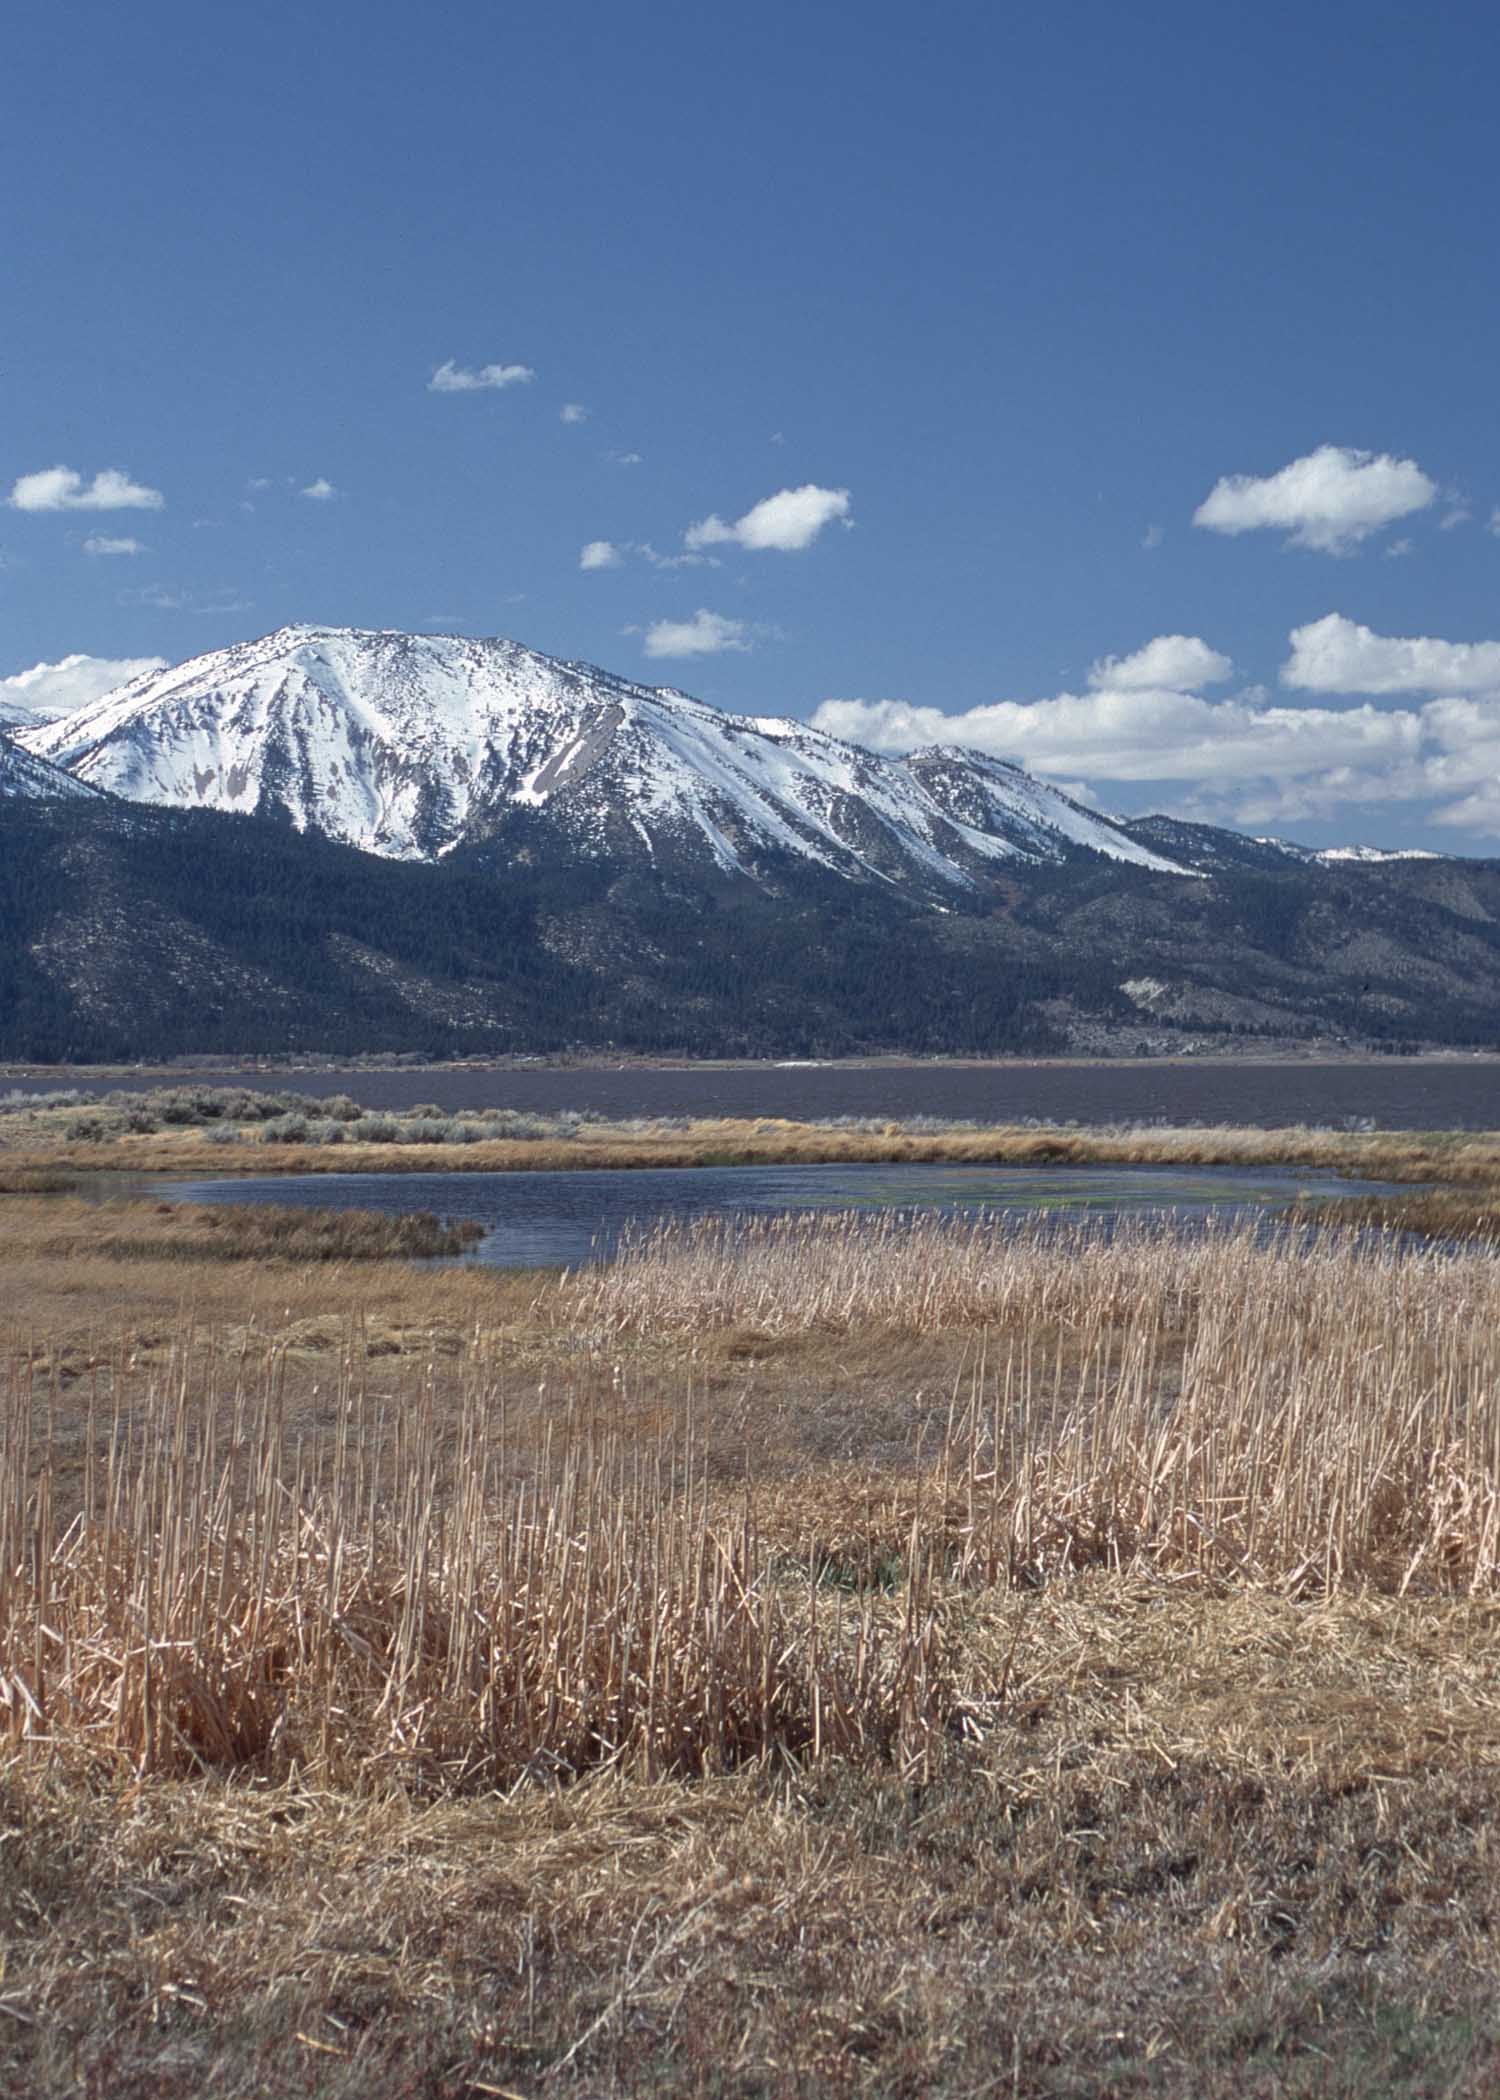
\includegraphics[width=\paperwidth,height=\paperheight]{photo.jpg}};

      \node (thuas) [shape=rectangle, fill=thuasgreen, minimum height=40mm, minimum width=\paperwidth, anchor=south west,opacity=0.5] at (current page.south west) {};
      \node[white] at (thuas.center) {\coverpagefontthuas De Haagse Hogeschool};

      \node (bar) [shape=rectangle, fill=thuasgrey, minimum width=\paperwidth, anchor=west, minimum height=1cm, opacity=0.8] at ([yshift=8cm]current page.south west) {};

      \node (student) at ([yshift=11cm,xshift=-1cm]current page.south east) {};
      \node[white,align=flush right,anchor=east] at (student.north east) {\coverpagefontstudent S. Tudent \\[2ex]\coverpagefontstudent 12345678\\[2ex]\coverpagefontstudent S.Tudent@student.hhs.nl\par};

      \node (opleiding) at ([yshift=6cm,xshift=-1cm]current page.south east) {};
      \node[white,align=flush right,anchor=east] at (opleiding.north east) {\coverpagefontopleiding Opleiding Civiele Techniek\par};

	  \node[white] (title) [align=center,text width=\paperwidth-8cm, anchor=north] at ([yshift=-3cm]current page.north) {\coverpagefonttitle\begin{hyphenrules}{nohyphenation} Watermanagement in droge omgevingen \end{hyphenrules}\par};

	  \node[white] (subtitle) [align=center,text width=\paperwidth-8cm, anchor=north] at ([yshift=-10cm]current page.north) {\coverpagefontisubtitle\begin{hyphenrules}{nohyphenation} --- Een innovatieve aanpak ---\end{hyphenrules}\par};
  \end{tikzpicture}

\newpage
\hspace*{0pt}

\vfill
\small{
	Deze scriptie is gemaakt in het kader van de afstudeerstage bij de opleiding Civiele Techniek.
	Aan deze scriptie kunnen geen rechten worden ontleend.

	Deze scriptie is tot stand gekomen met de medewerking van The Netherlands Water Partnership (\url{https://www.netherlandswaterpartnership.com/}).
}

\frontmatter
\chapter{Voorwoord}
\kant[1-2]
{\bigskip\hfill\slshape\ifcase \month \or Januari\or Februari\or Maart\or April\or Mei%
\or Juni\or Juli\or Augustus\or September\or October\or November\or December\fi\ \the\year, S. Tudent}
\tableofcontents
\chapter{Samenvatting}
\kant[1-2]

\mainmatter
\chapter{Inleiding}
\kant[1]
\section{More Kant}
\kant[1-6]

\chapter{Opdrachtsomschrijving}
\kant[7]
\section{More Kant}
\kant[8]

Zie figuur~\ref{fig:fig1}.

\begin{figure}[!ht]
\centering
\includegraphics[width=0.5\textwidth]{example-image-a}
\caption{This is an example of an image.}
\label{fig:fig1}
\end{figure}
\kant[9]

\chapter{Onderzoek}

\kant[1]
In~\eqref{equ:equ1} wordt aangegeven \ldots

In~\cite{oweis2003improving} wordt beschreven hoe de waterproductieviteit in \ldots\ kan worden verhoogd.

\begin{equation}
\label{equ:equ1}
\int_{0}^{\infty} \frac{1}{x}\ln x\, \mathrm{d}x = \ldots
\end{equation}

\begin{table}[!ht]
\centering
\caption{Meteorologische gegevens per stad in de maand juli 2017.}
\label{tab:my-table}
\begin{tabular}{@{}cccc@{}}
\toprule
Stad & Neerslag {[}mm{]} & Zonuren {[}h{]} & Temperatuur {[}C{]} \\ \midrule
A    & 25                & 36              & 19                  \\
B    & 23                & 40              & 21                  \\
C    & 21                & 25              & 20                  \\ \bottomrule
\end{tabular}
\end{table}

\backmatter

\bibliography{thesis_coverpage}

\end{document}
